\documentclass[10pt]{beamer}
\usetheme{jambro}

\title[]{Macroeconomia I - Modelo de 3 equações e política macroeconômica}
\author[]{\href{https://pvfonseca.github.io}{Paulo Victor da Fonseca}}
\date{}

\hypersetup{
    colorlinks = true,
    urlcolor = teal,
    linkcolor = teal    
}
\usepackage[portuguese]{babel}
\usepackage{subfig}
\usepackage{emoji}
\usepackage{hyperref}

\begin{document}

\begin{frame}[plain]
    \titlepage{
        \begin{center}
            \begin{minipage}{0.8\textwidth}
                \centering
            \end{minipage}
        \end{center}}
\end{frame}

\begin{frame}{Sumário}
    \tableofcontents
\end{frame}

\section{Introdução}
\begin{frame}
    {Introdução}
    \begin{enumerate}
        \item Como choques de DA produzem flutuações cíclicas no produto e emprego agregados\bigskip
        \item Características de lado de oferta determinam a inflação constante de equilíbrio\bigskip
        \item Combinação dos elementos de oferta e demanda agregadas
    \end{enumerate}
\end{frame}

\begin{frame}
    {Introdução}
    \begin{itemize}
        \item Isso produziu imagem de como economia é afetada por choques de OA e DA que são amplificados pelo processo multiplicador e amortecidos pela capacidade de famílias e firmas de se sustentarem via empréstimos quando renda corrente cai\bigskip
        \item Desemprego de equilíbrio (médio prazo): variações lentas e graduais\bigskip
        \item Desemprego efetivo, no entanto, aumenta ou diminui de acorco com ciclo econômico que é determinado, principalmente, por flutuações de DA\bigskip
        \item Na ausência de uma autoridade monetária ou intervenções de política macro de forma a impedir o hiato entre salário real que trabalhadores esperam assegurar (via curva WS) e salário real que firmas estão dispostas a pagar (curva PS), poderíamos ter um processo de espiral inflacionária quando desemprego está abaixo da taxa de equilíbrio (natural)
    \end{itemize}
\end{frame}

\begin{frame}
    {Introdução}
    \begin{itemize}
        \item A incompatibilidade entre reivindicações de firmas e trabalhadores - e, portanto, pressões inflacionárias - podem, em princípio, ser resolvidas por:\medskip
        \begin{enumerate}
            \item Mudanças institucionais ou políticas de oferta que aumentem o produto potencial (equilíbrio de médio prazo) - deslocando relação de WS para baixo, ou de PS para cima\medskip
            \item Uso de políticas de gerenciamento de DA para reduzir emprego e produto agregados a um nível consistente com o equilíbrio de médio prazo, quando inflação está constante. Este tipo de política toma instituições e políticas de oferta como dados\medskip
        \end{enumerate}
        \item Focaremos no segundo conjunto de medidas\bigskip
        \item Assumiremos que, inicialmente, economia esteja em equilíbrio de médio prazo (hiato do produto é zero e inflação constante)\bigskip
        \item Analisaremos como formulador de política deve responder a um choque que perturbe o equilíbrio inicial de forma a estabilizar a economia em seu nível de inflação constante
    \end{itemize}
\end{frame}

\begin{frame}
    {Introdução}
    \begin{itemize}
        \item Em resumo, \hlight{analisaremos em detalhe como uma política de gerenciamento de DA é implementada para estabilizar a economia}\bigskip
        \item Antes disso, discutiremos alguns detalhes acerca da implementação de regimes de metas de inflação e sua história recente\bigskip
        \item Durante a década de 1990s, muitos países adotaram um novo regime de política macro - \hlight{metas de inflação}\bigskip
        \item Governo delega a condução de política monetária e tarefa de estabilizar a economia a um Banco Central, adotando uma meta específica para a taxa anual de inflação\bigskip
        \item A meta mais comum adotada entre países desenvolvidos é de 2\% a.a.
    \end{itemize}
\end{frame}

\begin{frame}
    {Introdução}
    \begin{figure}
        \href{https://www.bcb.gov.br/estatisticas}{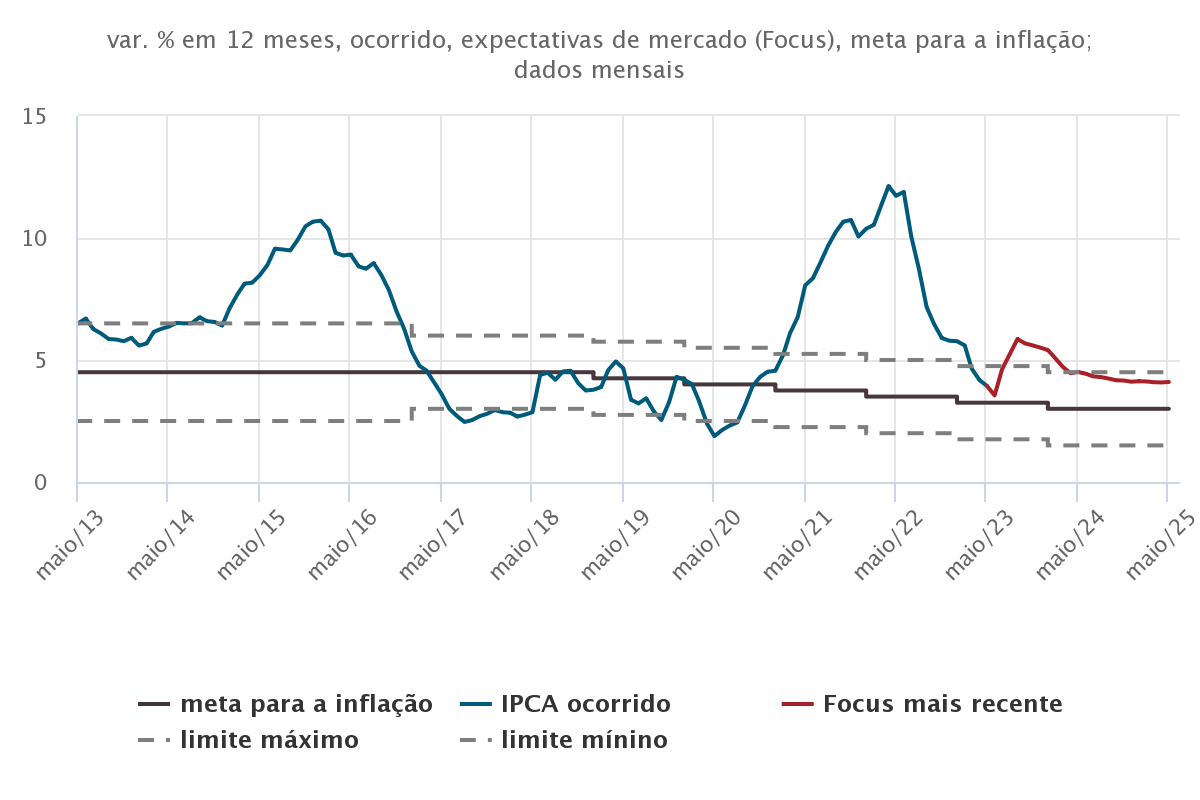
\includegraphics[width=.65\textwidth]{./figures/aula15_fig1.png}}
        \caption{\href{https://www.bcb.gov.br/estatisticas}{Metas de inflação - Brasil (2013 - 2025)}. Fonte: \href{https://www.bcb.gov.br/}{Banco Central do Brasil}}
    \end{figure}
\end{frame}

\begin{frame}
    {Introdução}
    \begin{itemize}
        \item Para entendermos porque essas mudanças no regime e condução de política foram adotadas, é útil focarmos em três questões:\medskip
        \begin{enumerate}
            \item Por que os governos, normalmente, definem as responsabildiades dos BC's como o controle da inflação?\medskip
            \item Por que os governos consideram a inflação um problema que precisa ser controlado?\medskip
            \item Por que os governos delegam a função de manter inflação baixa e estável aos formuladores de política monetária ao invés de controlarem a inflação eles mesmos?
        \end{enumerate}
    \end{itemize}
\end{frame}

\begin{frame}
    {Introdução}
    \begin{itemize}
        \item Primeira questão: a taxa de desemprego para a qual a inflação é constante depende de características estruturais dos mercados de trabalho e de bens e serviços\bigskip
        \item Essas características determinam as posições das curvas WS e PS\bigskip
        \item Mas como os BCs não possuem instrumentos de política que permitam influenciar características de lado de oferta, claramente, não são os formuladores de política apropriados para reduzir o desemprego de equilíbrio (natural) em uma economia\bigskip
        \item Caso seja este o objetivo, deverá ser alcançado pelo próprio governo com políticas de oferta
    \end{itemize}
\end{frame}

\begin{frame}
    {Introdução}
    \begin{itemize}
        \item Existe, no entanto, outra forma pelo qual o BC consegue influenciar desemprego\bigskip
        \item Um BC com responsabilidade de manter um nível elevado de emprego e, ao mesmo tempo, manter taxa de inflação próxima à meta estipulada estará menos inclinado a acomodar bruscas políticas anti-inflacionárias ao permitir uma rápida elevação da taxa de desemprego\bigskip
        \item O modelo de 3 equações permite a representação de variadas formas de comportamento de diferentes BCs ao redor do mundo
    \end{itemize}
\end{frame}

\begin{frame}
    {Introdução}
    \begin{itemize}
        \item \hlight{Por que formuladores de política se preocupam com inflação?}\bigskip
        \item Um dos motivos imediatos para manter inflação baixa: nível de inflação é uma das principais prioridades para eleitores\bigskip
        \item Governos podem ter que pagar um preço eleitoral elevado se não conseguirem manter inflação sob controle\bigskip
        \item A importância que o público geral norte-americano dá à inflação é analisada em um artigo de Shiller de 1997: \emph{survey} de economistas e público geral sobre suas visões acerca da inflação\bigskip
        \item O resultado mostra que o público geral (mais que economistas) veem o controle da inflação como uma prioridade nacional
    \end{itemize}
\end{frame}

\begin{frame}
    {Introdução}
    \begin{figure}
        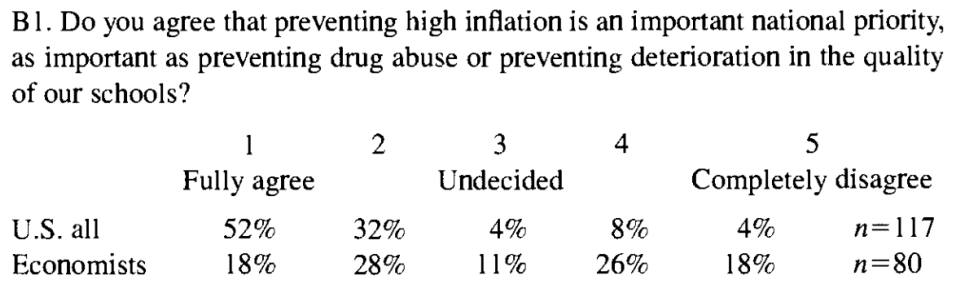
\includegraphics[width=\textwidth]{./figures/aula15_fig2.png}
        \caption{Atitudes do público com relação à importância de evitar inflação elevada. Fonte: Shiller (1997)}
    \end{figure}
\end{frame}

\begin{frame}
    {Introdução}
    \begin{itemize}
        \item \hlight{Por que, em um regime de metas de inflação, a política de estabilização é delegada à autoridade monetária?}\bigskip
        \begin{enumerate}
            \item \textcolor{blue}{Por que o instrumento primário de política de estabilização é a política monetária, e não a política fiscal?}\medskip
            \begin{itemize}
                \item Razões práticas e políticas para isso\medskip
                \item Variações tributárias ou de gastos públicos, normalmente, envolvem processos parlamentares demorados, e não há um equivalente ao ajuste gradual possível via mudanças na taxa básica de juros em intervalos mensais\medskip
                \item Além disso, política fiscal é inerentemente política, dado que envolve o uso de receitas tributárias: "\emph{Nenhuma tributação sem representação} (slogan política com origem na Revolução Americana)\medskip
                \item Política monetária é vista como mais neutra que a fiscal e não cria ganhadores ou perdedores óbvios, tornando-a um instrumento de política menos controverso para uso no gerenciamento de curto prazo de DA
            \end{itemize}
        \end{enumerate}        
    \end{itemize}
\end{frame}

\begin{frame}
    {Introdução}
    \begin{enumerate}
        \item[2] \textcolor{blue}{Por que o governo delega a condução de política monetária para um BC independente?}\medskip
        \begin{itemize}
            \item Governo pode obter ganhos eleitorais com controle da política monetária: aumentar PIB acima do potencial ou alterar taxas de juros específicas diante de uma eleição\medskip
            \item No entanto, como governos não dispõem de credibilidade de manter inflação baixa, isso traduz-se em inflação mais alta\medskip
            \item A pressão política para manipular taxas de juros (ou estimular produto/reduzir desemprego) é a fonte deste déficit de credibilidade\medskip
            \item BCs independentes não sofrem essas pressões e, portanto, é mais provável que consigam atingir uma inflação mais baixa e estável\medskip
            \item Como eleitores se importam com inflação e gerenciamentos macroeconômicos sólidos, isso gera incentivo para governo delegar a condução da política monetária
        \end{itemize} 
    \end{enumerate}
\end{frame}

\section{Papel do BC na estabilização}
\begin{frame}
    {Papel do BC na estabilização}
    \begin{itemize}
        \item Desde o começo dos anos 1990, um número crescente de BCs assumiu a responsabilidade de estabilizar a macroeconomia ao redor de uma meta de taxa de inflação baixa\bigskip
        \item \hlight{Regime de metas de inflação}\bigskip
        \item Em resposta a um aumento inflacionário, espera-se que o BC aumente a taxa de juros\bigskip
        \item Isso reduziria gastos que são sensíveis a variações na taxa de juros (e.g., gastos com imóveis, bens duráveis, máquinas e equipamentos)\bigskip
        \item A redução no investimento e consumo, por sua vez, levaria a uma contração de DA e uma queda no produto agregado\bigskip
        \item Desemprego aumentaria e, por fim, a pressão inflacionária seria reduzida
    \end{itemize}
\end{frame}

\begin{frame}
    {Papel do BC na estabilização}
    \begin{itemize}
        \item Em 1997, ano em que o Bank of England tornou-se independente, o economista-chefe do BoE, Mervyn King (mais tarde tornou-se Diretor - \emph{Governor}) explicou:\bigskip        
    \end{itemize}
    \begin{quote}
        A política monetária pode ser descrita em termos de duas variáveis de política - uma meta de inflação de médio prazo e uma resposta das taxas de juros a choques que criam flutuações na inflação e no produto agregado. O objetivo primordial da política monetária é assegurar que, em média, a inflação é igual à meta. Mas essa meta não é suficiente para definir a política. Existe uma decisão subordinada de como responder a choques à medida que estes ocorrem.
    \end{quote}
    \begin{flushright}
        (\href{https://en.wikipedia.org/wiki/Mervyn_King,_Baron_King_of_Lothbury}{Mervyn King}, 1997)
    \end{flushright}
\end{frame}

\begin{frame}
    {Papel do BC na estabilização}
    \begin{figure}
        \href{https://bookdown.org/robohay/economicsnotes/Figures/Policy/BoEFig.jpg}{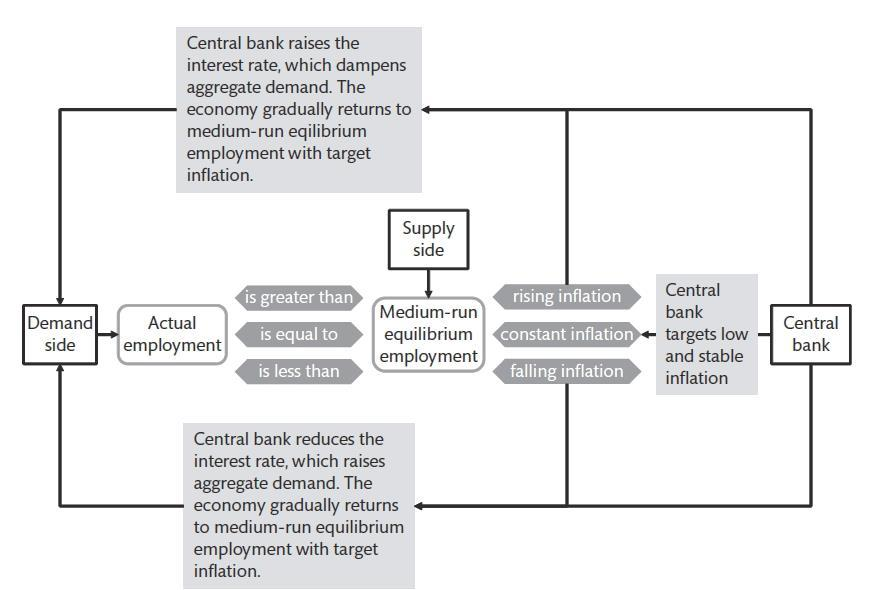
\includegraphics[width=.65\textwidth]{./figures/aula15_fig3.jpg}}
        \caption{Visão esquemática do modelo macro. Fonte: \href{https://bookdown.org/robohay/economicsnotes/Figures/Policy/BoEFig.jpg}{Carlin e Soskice (2015)}}
    \end{figure}
\end{frame}

\begin{frame}
    {Papel do BC na estabilização}
    \begin{itemize}
        \item Figura com visão esquemática do modelo macro, incluindo autoridade monetária\bigskip
        \item Lado esquerdo: resumo dos lados de DA e OA\bigskip
        \item Componentes de DA determinam nível de emprego e produto no equilíbrio do mercado de bens\bigskip
        \item Características estruturais de lado de oferta determinam taxa de desemprego de equilíbrio de médio prazo, ao qual a taxa de inflação é constante\bigskip
        \item Terceiro painel: implicações para taxa de inflação\bigskip
        \item Flechas externas mostram o \emph{feedback} da regra de política monetária do BC à DA\bigskip
        \item Ilustração de como o BC usa uma regra de política monetária para manter inflação efetiva próxima à meta
    \end{itemize}
\end{frame}

\begin{frame}
    {Papel do BC na estabilização}
    \begin{figure}
        \href{https://www.bcb.gov.br/content/controleinflacao/Infograficos_controleinflacao/VF_ajuste_info_canais_de_transmissao_da_politica_monetaria_br_0509_2021.png}{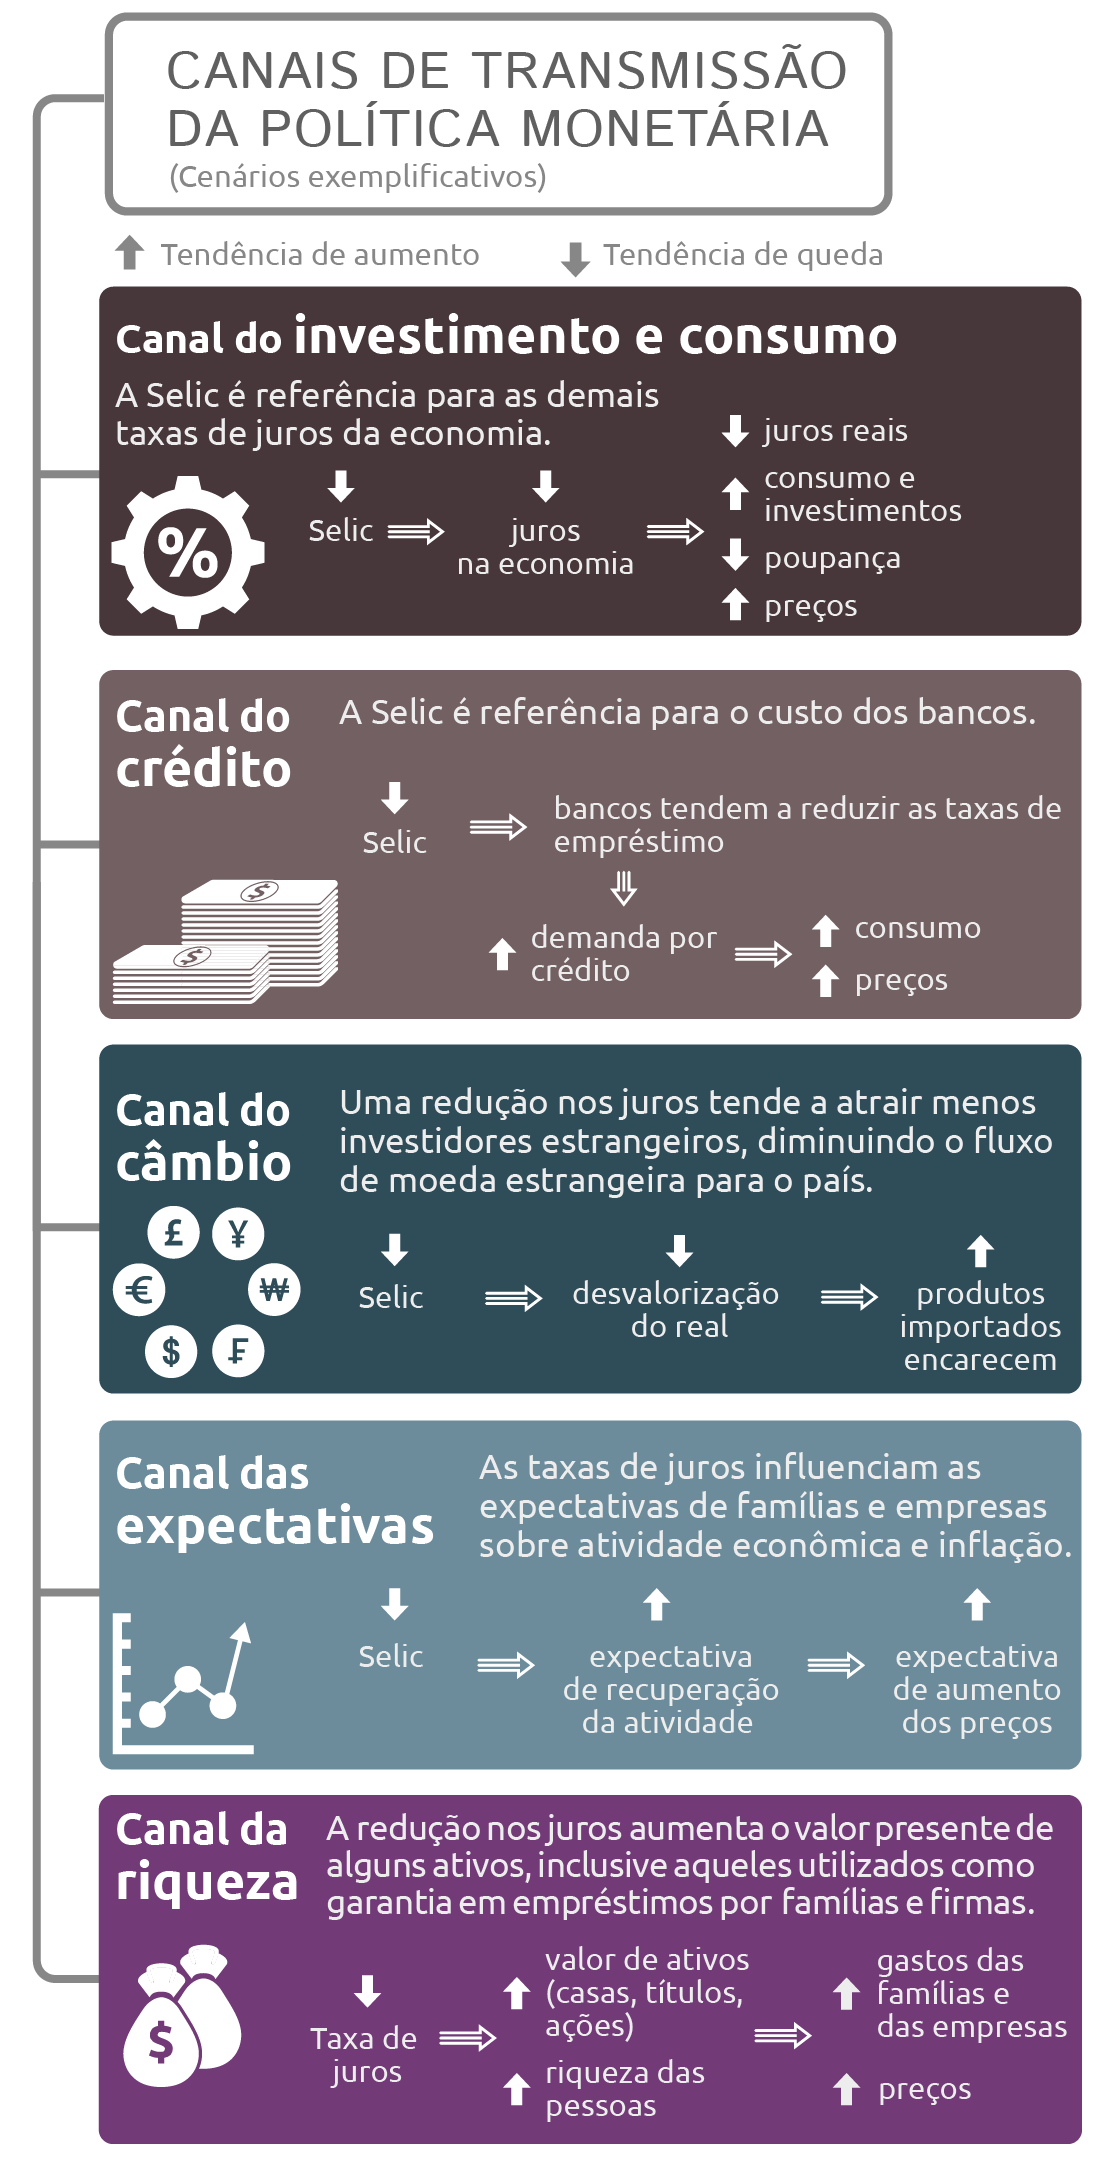
\includegraphics[width=.23\textwidth]{./figures/aula15_fig4.png}}
        \caption{Canais de transmissão da política monetária. Fonte: \href{https://www.bcb.gov.br/content/controleinflacao/Infograficos_controleinflacao/VF_ajuste_info_canais_de_transmissao_da_politica_monetaria_br_0509_2021.png}{Banco Central do Brasil}}
    \end{figure}
\end{frame}

\begin{frame}
    {Papel do BC na estabilização}
    \begin{figure}
        \href{https://www.bcb.gov.br/content/controleinflacao/Infograficos_controleinflacao/Info-Controle-politicamonetariaeomeubolso-v2.png}{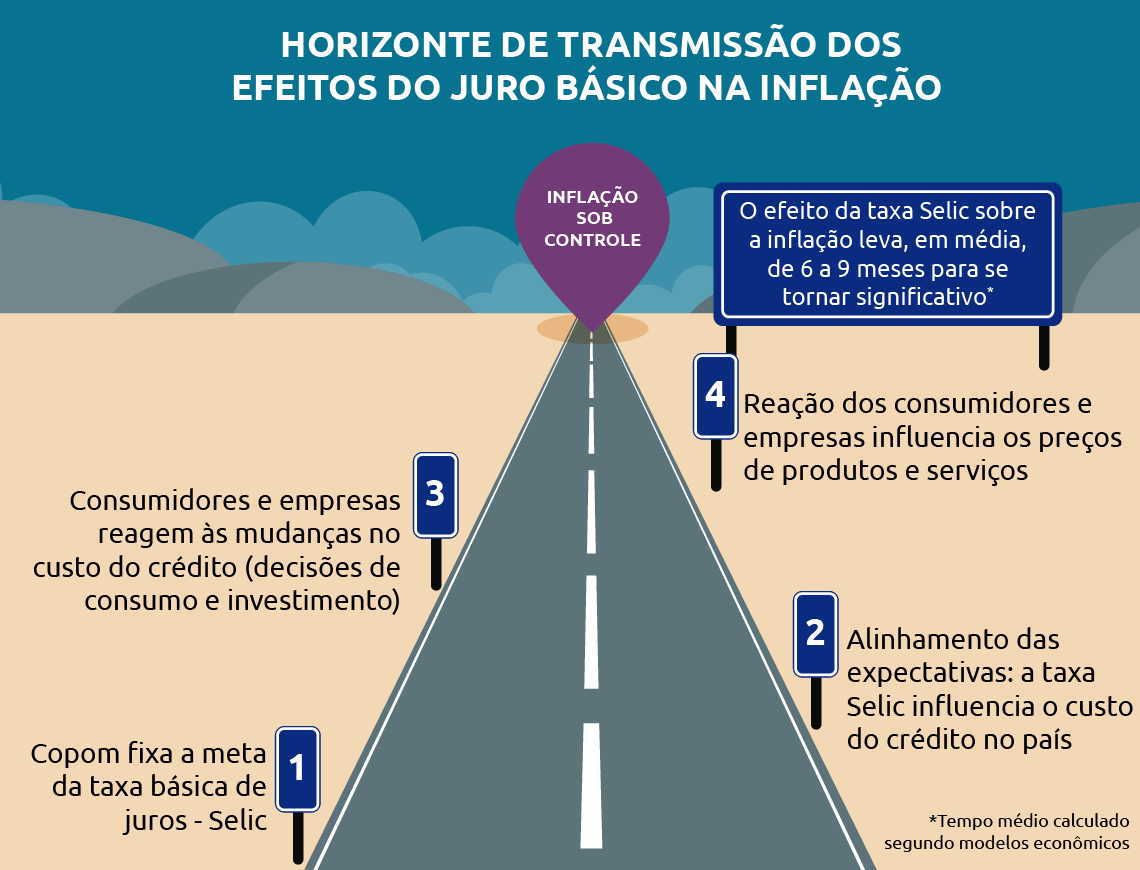
\includegraphics[width=.6\textwidth]{./figures/aula15_fig5.png}}
        \caption{Horizonte de transmissão da política monetária. Fonte: \href{https://www.bcb.gov.br/content/controleinflacao/Infograficos_controleinflacao/Info-Controle-politicamonetariaeomeubolso-v2.png}{Banco Central do Brasil}}
    \end{figure}
\end{frame}

\begin{frame}
    {Papel do BC na estabilização}
    \begin{figure}
        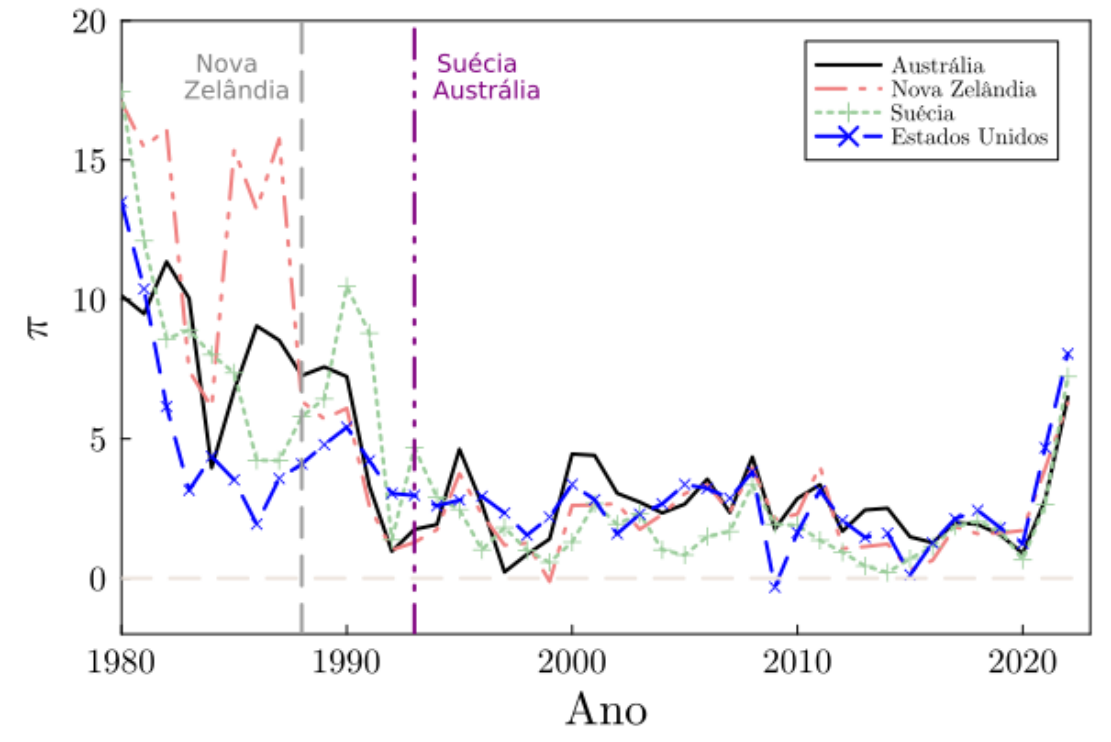
\includegraphics[width=.6\textwidth]{./figures/aula15_fig6.PNG}
        \caption{Taxas de inflação - antes e depois adoção de metas de inflação: 1980-2022. Fonte: \href{https://www.imf.org/en/Publications/SPROLLS/world-economic-outlook-databases\#sort=\%40imfdate\%20descending}{FMI - World Economic Outlook}}
    \end{figure}
\end{frame}

\begin{frame}
    {Papel do BC na estabilização}
    \begin{itemize}
        \item Figura anterior mostra trajetórias de inflação em uma seleção de economias desenvolvidas desde 1980\bigskip
        \item Período de inflação elevada e volátil foi seguida por um período de inflação baixa e estável\bigskip
        \item A introdução dos regimes de metas de inflação foi parte da evolução de um arcabouço de políticas econômicas sob os quais, a partir do final de 1970, os governos usaram políticas econômicas para combate à inflação via depressão de DA\bigskip
        \item A mudança para um regime de baixa inflação iniciou-se antes da grande queda nos preços do petróleo em 1986 e da gradual emergência de manufaturados de baixo custo (espcialmente chineses) nos mercados mundiais que, subsequentemente, também tiveram efeito significativo sobre a inflação
    \end{itemize}
\end{frame}

\begin{frame}
    \begin{itemize}
        \item Apesar de um regime formal de metas de inflação não ter sido adotado pelo Fed até recentemente, o comportamento da taxa de inflação foi similar ao observado nos outros países\bigskip
        \item A mudança para um regime de metas de inflação, formal ou informal, é frequentemente identificado com o começo do período de \hlight{Grande Moderação} (período de estabilidade macroeconômica sem precedentes)
    \end{itemize}
\end{frame}

\begin{frame}
    {Papel do BC na estabilização}
    \begin{figure}
        \href{https://bookdown.org/robohay/economicsnotes/Figures/Demand/gtmoderation.jpg}{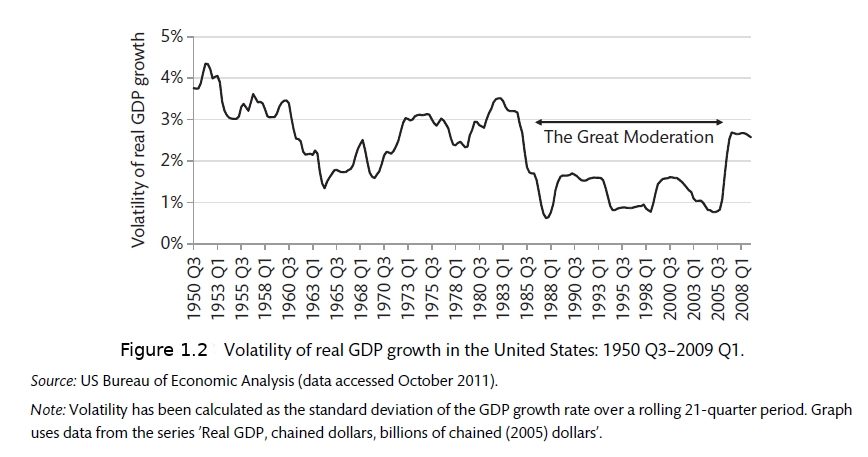
\includegraphics[width=.8\textwidth]{./figures/aula15_fig7.jpg}}
        \caption{Volatilidade do crescimento do PIB real - EUA (1950.3 - 2009.1). Fonte: \href{https://bookdown.org/robohay/economicsnotes/Figures/Demand/gtmoderation.jpg}{Carlin e Soskice (2015)}}
    \end{figure}
\end{frame}

\begin{frame}
    {Papel do BC na estabilização}
    \begin{figure}
        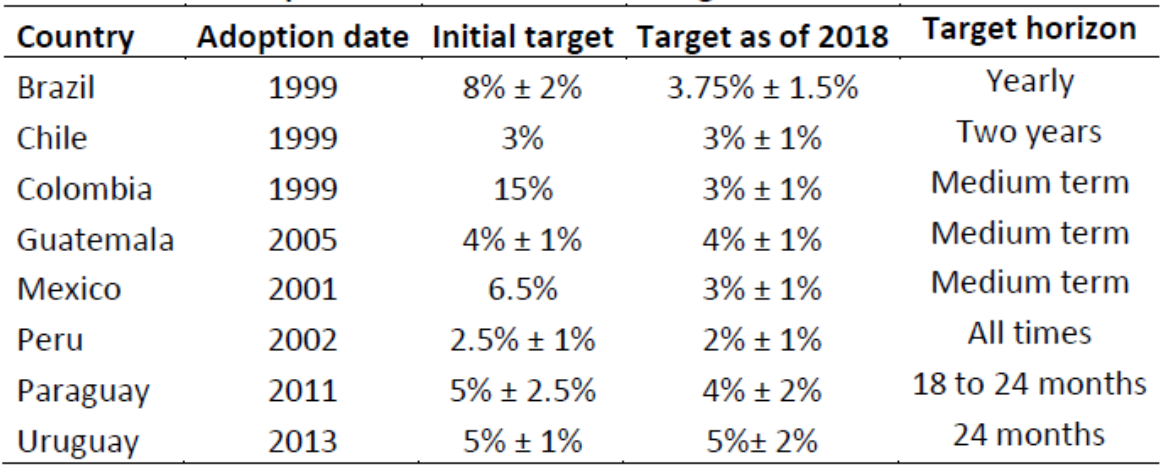
\includegraphics[width=.9\textwidth]{./figures/aula15_fig8.PNG}
        \caption{Data de implementação e metas de inflação - América Latina. Fonte: De Gregorio (2019)}
    \end{figure}
\end{frame}

\begin{frame}
    {Papel do BC na estabilização}
    \begin{figure}
        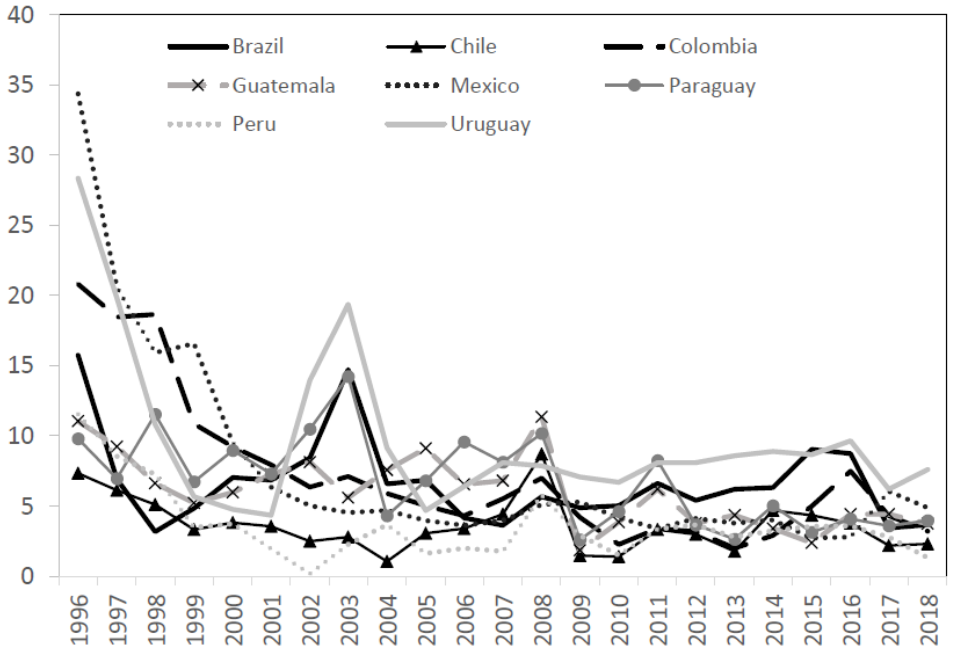
\includegraphics[width=.65\textwidth]{./figures/aula15_fig9.PNG}
        \caption{Inflação - América Latina. Fonte: De Gregorio (2019)}
    \end{figure}
\end{frame}

\begin{frame}
    {Papel do BC na estabilização}
    \begin{figure}
        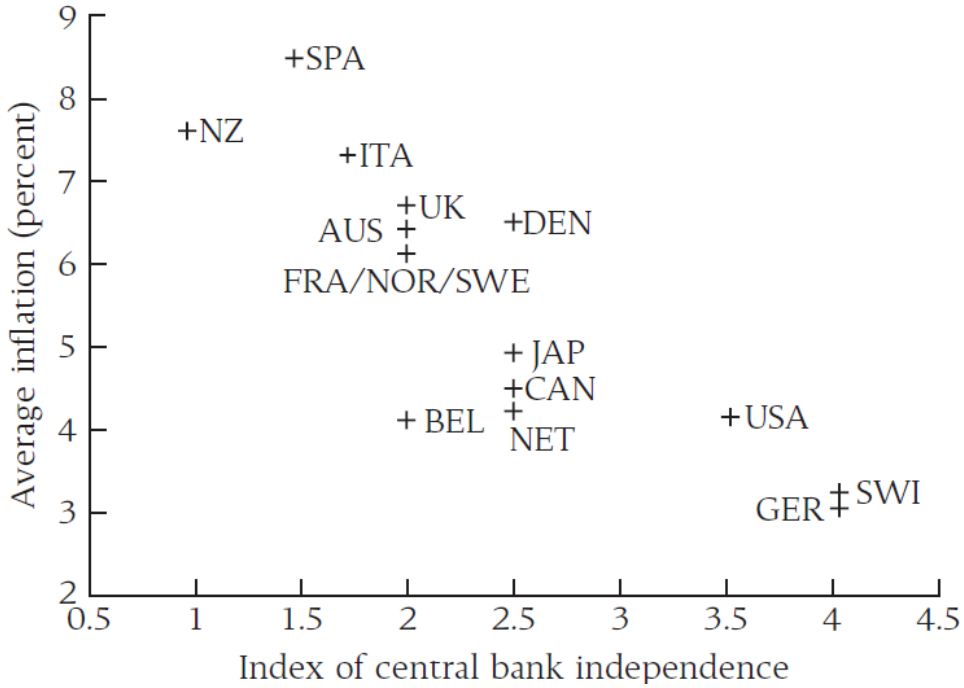
\includegraphics[width=.6\textwidth]{./figures/aula15_fig10.PNG}
        \caption{Independência do Banco Central $\times$ inflação. Fonte: Romer (2018)}
    \end{figure}
\end{frame}

\begin{frame}
    {Papel do BC na estabilização}
    \begin{itemize}
        \item Duas situações importantes nas quais o BC não pode depender apenas de variações da taxa de juros para estabilizar economia frente a choques\bigskip
        \begin{enumerate}
            \item \hlight{Limite inferior da taxa de juros}\medskip
            \begin{itemize}
                \item Choque adverso de DA tão significativo que mesmo quando o BC reduz taxa nominal para zero, este valor não é baixo o suficiente para estimular uma recuperação da DA\medskip
                \item Com taxa de juros nominal em zero (ou no limite inferior efetivo), a taxa de juros real - variável relevante para decisões de investimento - não é baixa o suficiente para estimular gastos que são sensíveis à taxa de juros\medskip
                \item Problema de ZLB é intimamente ligado à possibilidade de que economia possa entrar em uma \textcolor{purple}{armadilha deflacionária}, ciclo vicioso de queda no produto agregado e inflação\medskip
                \item Uma vez que canais convencionais estão inoperantes, BC pode tentar estimular economia usando políticas não-convencionais (\emph{quantitative easing, forward-guidance}), ou pode dividir responsabilidades de estabilização com política fiscal
            \end{itemize}
        \end{enumerate}
    \end{itemize}
\end{frame}

\begin{frame}
    {Papel do BC na estabilização}
    \begin{enumerate}
        \item[2] \hlight{Taxa de câmbio fixo}\medskip
        \begin{itemize}
            \item Observável em arranjos monetários de área monetária comum, como a Zona do Euro: países membros adotam euro como moeda e compartilham uma única autoridade monetária, o Banco Central Europeu (ECB)\medskip
            \item Como resultado, estes países não possuem suas próprias autoridades monetárias que poderiam estabilizar choques países-específicos\medskip
            \item Como todos os países da Zona do Euro possuem a mesma política monetária, qualquer política de estabilizaçãod e choques em um país em particular deve ser atingida via uso de política fiscal
        \end{itemize}
    \end{enumerate}
\end{frame}

\section{Inflação e deflação}
\begin{frame}
    {Inflação crescente e conflito distributivo}
    \begin{itemize}
        \item Inflação crescente reflete conflito distributivo, à medida que grupos sociais distintos (fixadores de salários/empregados e fixadores de preços/empregadores) buscam proteger seus próprios interesses\bigskip
        \item Quando grupos como sindicatos podem influenciar salários nominais e firmas possuem poder de determinação de preços, uma situação de inflação crescente reflete demandas inconsistentes destes grupos sobre o produto \emph{per capita} produzido pela economia\bigskip
        \item I.e., quando desemprego está abaixo da taxa natural, o hiato entre curvas WS e PS reflete conflito distributivo e leva a um aumento da inflação\bigskip
        \item Com desemprego baixo, trabalhadores têm mais poder de barganha e são capazes de assegurar um salário real mais elevado\bigskip
        \item Firmas tentarão manter margens de lucro fixando preços de forma apropriada - criando um hiato entre o salário real esperado mais elevado na curva WS e o salário real inalterado na curva PS
    \end{itemize}
\end{frame}

\begin{frame}
    {Inflação crescente e conflito distributivo}
    \begin{itemize}
        \item Lógica similar pode ser usada em arcabouço de salário eficiência\bigskip
        \item O conflito de interesses entre os dois lados do mercado de trabalho significa que o salário que empregadores precisam pagar para extrair maior esforço dos trabalhadores (dado o estado do mercado de trabalho) pode diferir do salário real compatível com a margem de lucros desejada pela firma\bigskip
        \item Desemprego baixo diminui o custo de perda de empregos e aumenta o salário eficiência\bigskip
        \item Aumentando, então, a taxa de inflação
    \end{itemize}
\end{frame}

\begin{frame}
    {Inflação crescente e conflito distributivo}
    \begin{itemize}
        \item Inflação crescente produz tensão social\bigskip
        \item Episódios inflacionários frequentemente são seguidos por períodos de \hlight{desinflação} custosos, períodos de produto abaixo do potencial (desemprego elevado) são necessários para reduzir inflação\bigskip
        \item Evidência empírica sugere que períodos de desinflação para reduzir a inflação a taxas moderadas (até dois dígitos a.a.) envolvem custos significativos em economias da OCDE onde isso aconteceu\bigskip
        \item Figura a seguir: trajetórias de inflação e desemprego no UK de 1971-2021\bigskip
        \item Período de inflação alta dos anos 70 foi combatido com apertos de política monetária\bigskip
        \item A redução da inflação de taxas acima de 20\% para abaixo de 5\% foi associada a um aumento no desemprego de 4\% para 12\% durante o período desinflacionário
    \end{itemize}
\end{frame}

\begin{frame}
    {Inflação crescente e conflito distributivo}
    \begin{figure}
        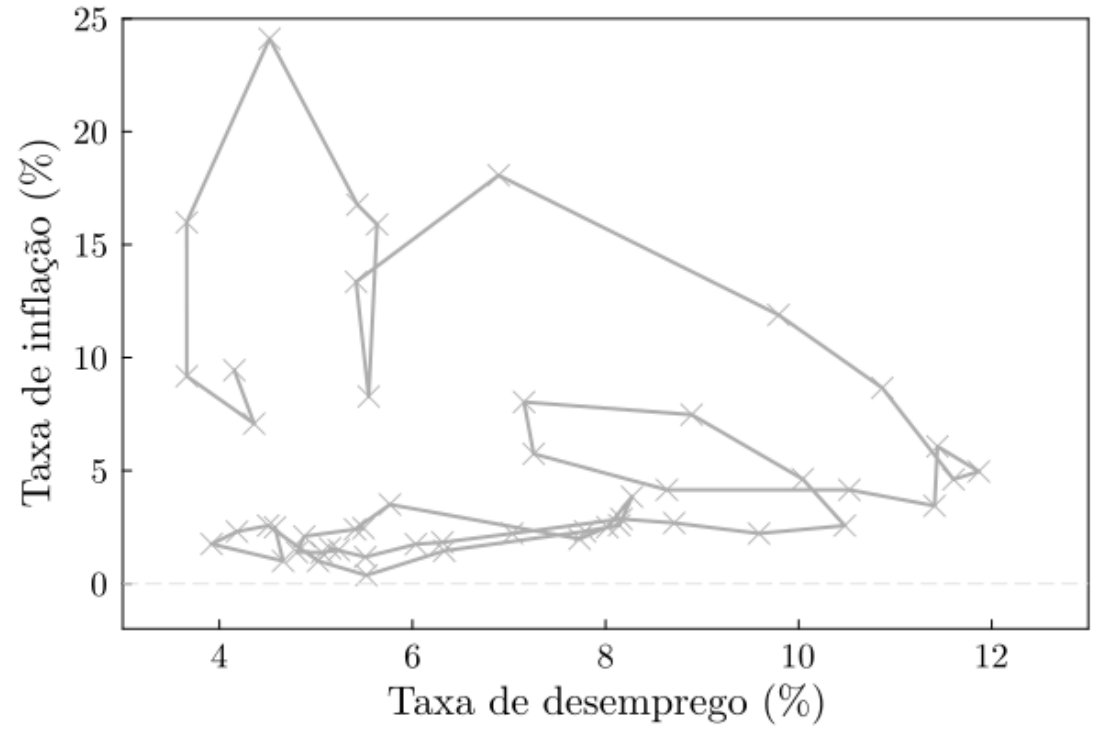
\includegraphics[width=.65\textwidth]{./figures/aula15_fig11.PNG}
        \caption{Inflação e desemprego: UK 1971-2021. Fonte: Elaboração própria}
    \end{figure}
\end{frame}

\begin{frame}
    {Inflação crescente e conflito distributivo}
    \begin{figure}
        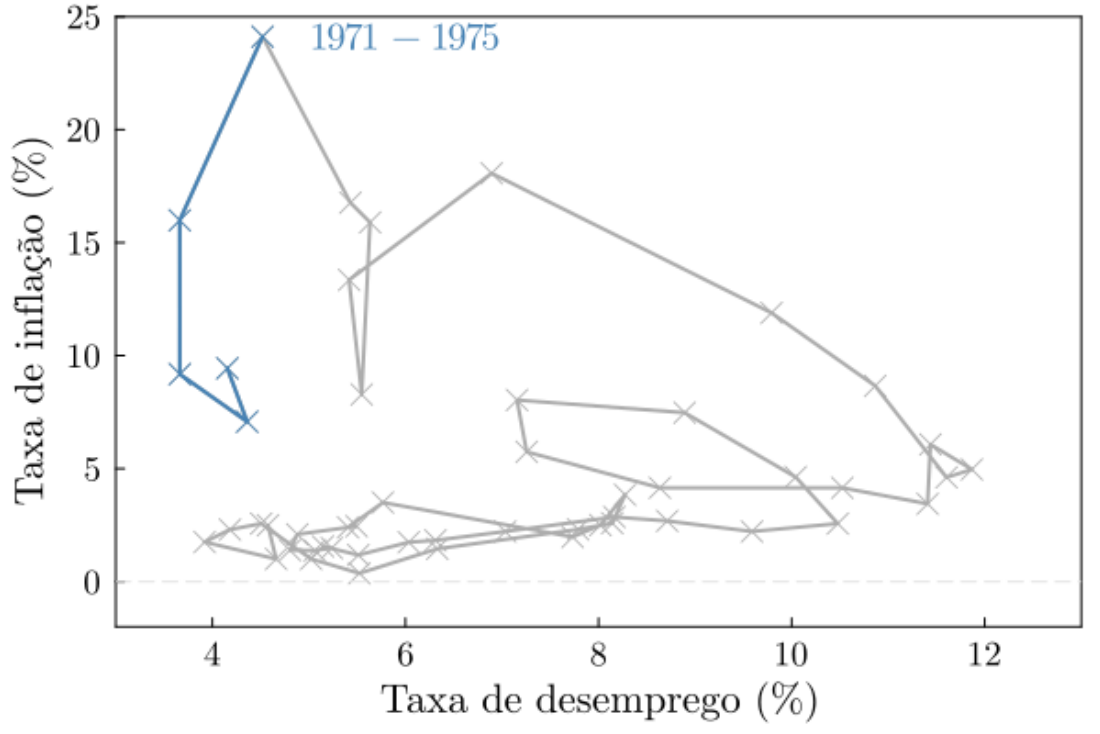
\includegraphics[width=.65\textwidth]{./figures/aula15_fig12.PNG}
        \caption{Inflação e desemprego: UK 1971-2021. Fonte: Elaboração própria}
    \end{figure}
\end{frame}

\begin{frame}
    {Inflação crescente e conflito distributivo}
    \begin{figure}
        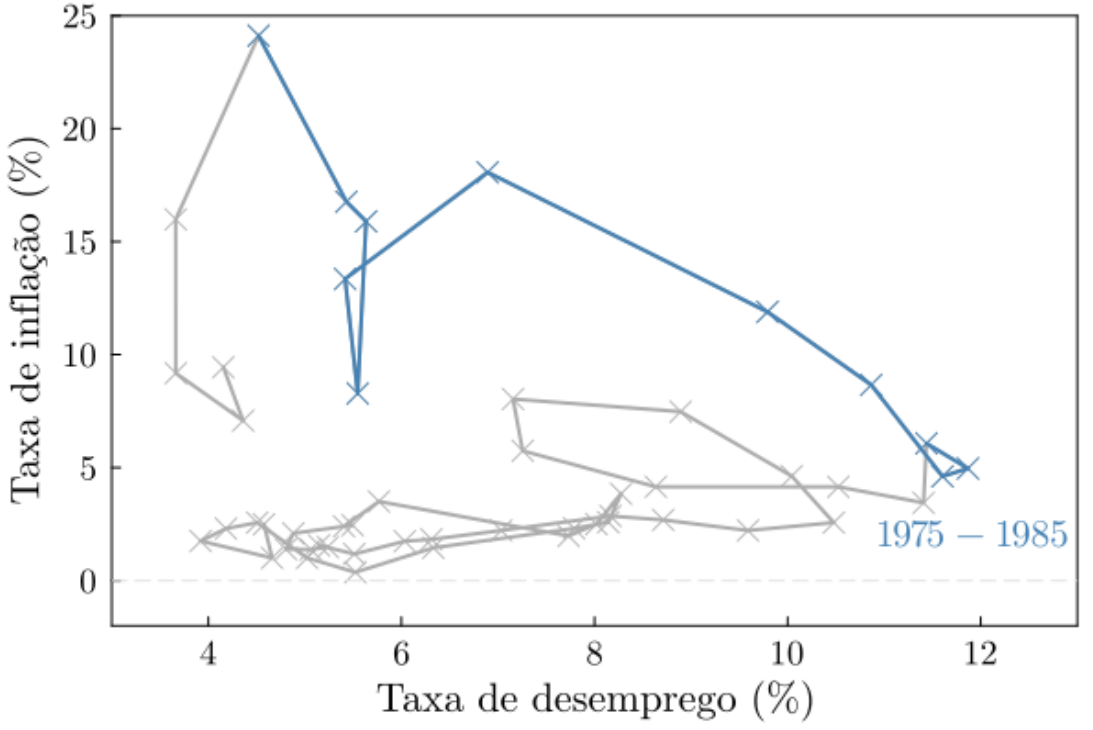
\includegraphics[width=.65\textwidth]{./figures/aula15_fig13.PNG}
        \caption{Inflação e desemprego: UK 1971-2021. Fonte: Elaboração própria}
    \end{figure}
\end{frame}

\begin{frame}
    {Inflação crescente e conflito distributivo}
    \begin{figure}
        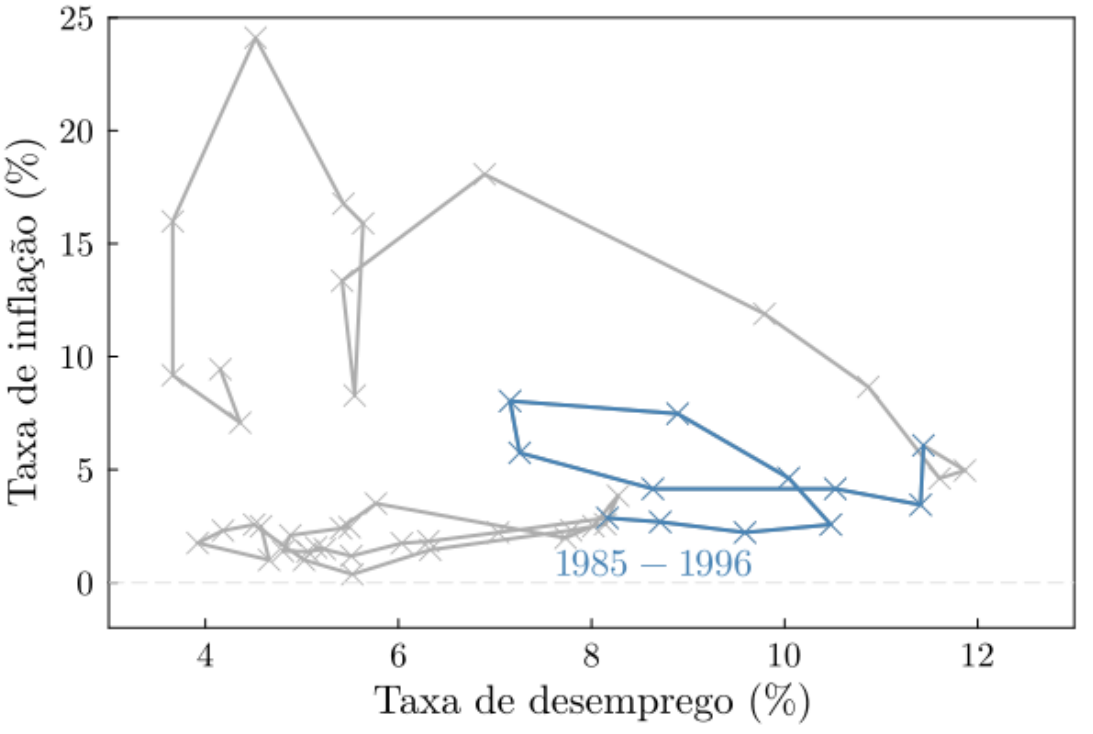
\includegraphics[width=.65\textwidth]{./figures/aula15_fig14.PNG}
        \caption{Inflação e desemprego: UK 1971-2021. Fonte: Elaboração própria}
    \end{figure}
\end{frame}

\begin{frame}
    {Inflação crescente e conflito distributivo}
    \begin{figure}
        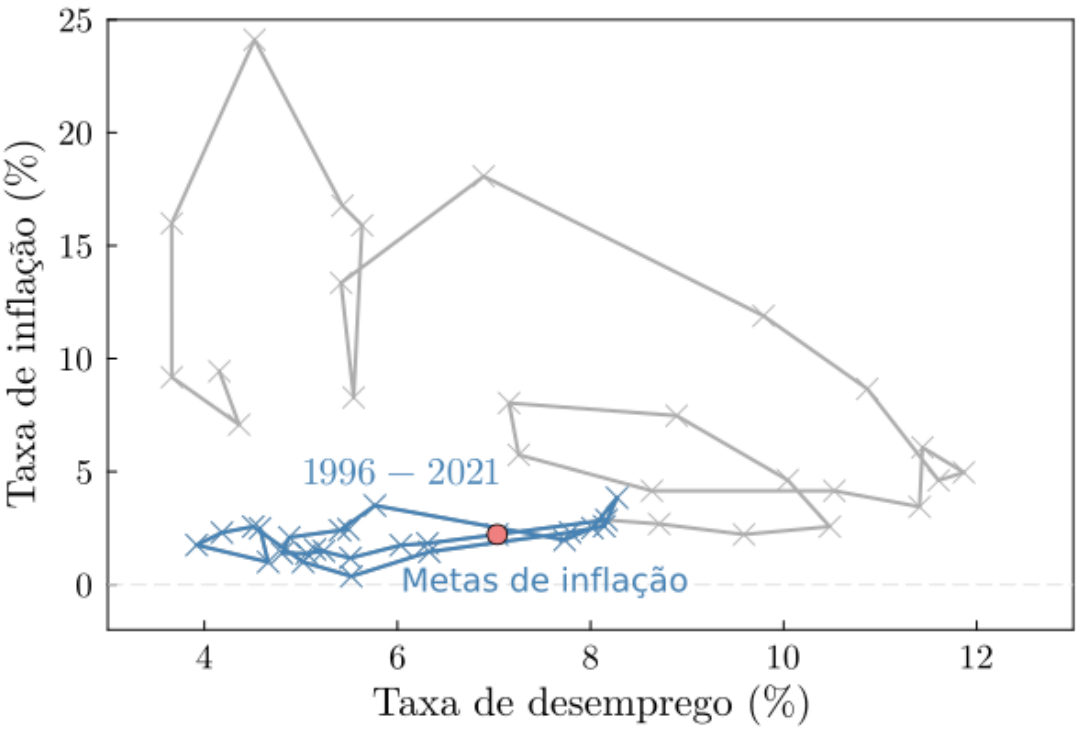
\includegraphics[width=.65\textwidth]{./figures/aula15_fig15.PNG}
        \caption{Inflação e desemprego: UK 1971-2021. Fonte: Elaboração própria}
    \end{figure}
\end{frame}

\begin{frame}
    {Inflação baixa e estável: benefícios}
    \begin{figure}
        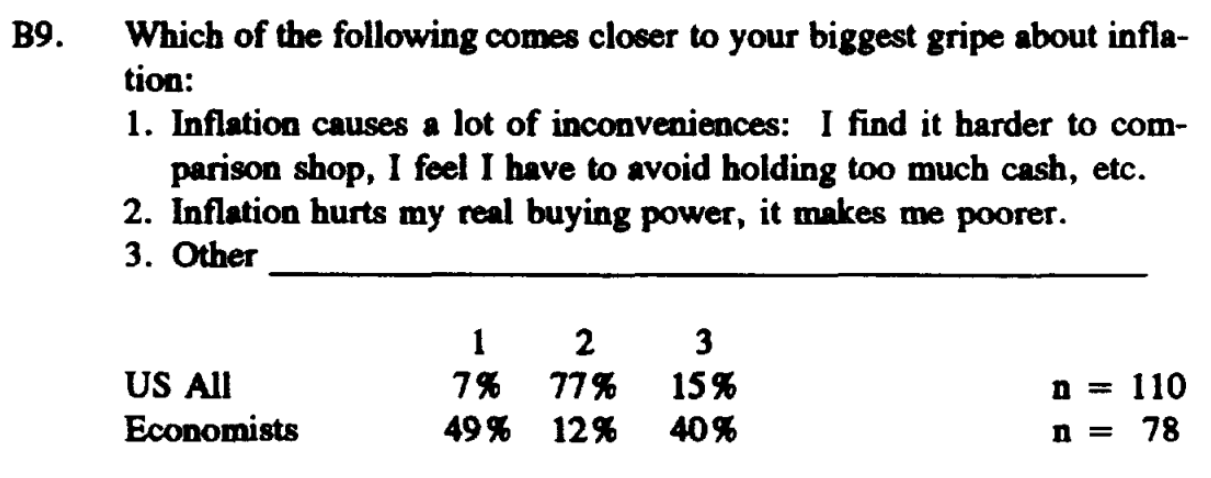
\includegraphics[width=\textwidth]{./figures/aula15_fig16.PNG}
        \caption{Qual a maior queixa com relação à inflação? Fonte: Shiller (1997)}
    \end{figure}
\end{frame}

\begin{frame}
    {Inflação baixa e estável: benefícios}
    \begin{itemize}
        \item Principal motivo pelo qual a população dos EUA tem aversão à inflação é devido à erosão do padrão de vida que acredita-se acompanhar uma inflação elevada\bigskip
        \item Relacionando ao modelo desenvolvido de lado de oferta, a maior queixa com relação à inflação tem a ver com o resultado do modelo WS-PS em ambiente inflacionário: inflação crescente leva a uma frustração persistente das expectativas de salários reais dos trabalhadores\bigskip
        \item No modelo que desenvolvemos, usamos o caso simples de protocolo temporal de fixação de preços e salários\bigskip
        \item Se firmas são capazes de ajustar preços imediatamente após a fixação de salários, uma inflação crescente reflete em uma situação na qual a demanda por salários reais são sistematicamente frustradas (o salário real esperado por trabalhadores, como indicado por WS, está acima do salário real vigente - que está sobre a curva PS)
    \end{itemize}
\end{frame}

\begin{frame}
    {Inflação baixa e estável: benefícios}
    \begin{itemize}
        \item No entanto, se há hiatos tanto na determinação de preços quanto de salários, o salário real estará entre as curvas WS e PS\bigskip
        \item Neste caso, nem fixadores de preços nem de salários estarão completamente satisfeitos\bigskip
        \item Este caso é mais realista: evidência empírica sugere que salários reais são levemente pró-cíclicos - figura a seguir\bigskip
        \item Ou seja, quando o hiato do produto é positivo, o salário real está entre as curvas WS e PS (i.e., maior que o valor de equilíbrio de inflação constante)
    \end{itemize}
\end{frame}

\begin{frame}
    {Inflação baixa e estável: benefícios}
    \begin{figure}
        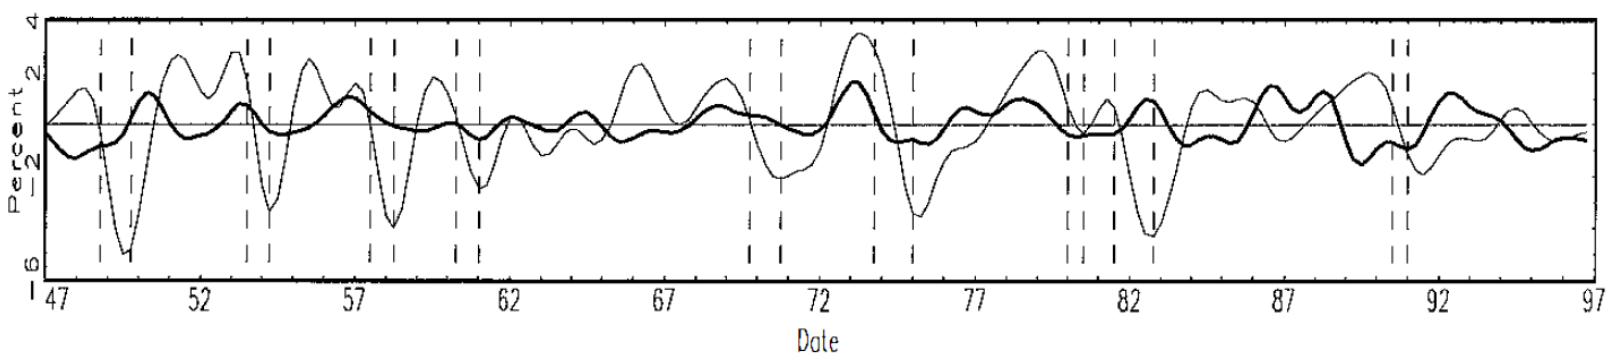
\includegraphics[width=\textwidth]{./figures/aula15_fig17.PNG}
        \caption{Salário real $\times$ PIB real - EUA (1947-1996). Fonte: Stock e Watson (1999)}
    \end{figure}
\end{frame}

\begin{frame}
    {Inflação baixa e estável: benefícios}
    \begin{itemize}
        \item Tabela anterior: divergências entre opinião pública e economistas com relação aos custos mais significativos da inflação\medskip
        \item Público geral: erosão do poder de compra\medskip
        \item Economistras: interferência que inflação elevada cria sobre habilidades dos preços em refletir informações\medskip
        \item Períodos de inflação alta são, frequentemente, de inflação mais volátil\medskip
        \item Considere economia com progresso tecnológico onde inovação acontece de maneira assimétrica entre setores\medskip
        \item Setores mais inovadores apresentarão preços decrescentes relativamente a setores com inovação mais estagnada\medskip
        \item Estas são mudanças economicamente consideráveis em preços relativos e, portanto, deveria levar a realocações de recursos\medskip
        \item Uma inflação mais volátil pode distorcer a alocação de recursos: mais difícil extrair sinais de mudanças de preços relativos $\times$ preços absolutos
    \end{itemize}
\end{frame}

\begin{frame}
    {Inflação baixa e estável: benefícios}
    \begin{itemize}
        \item Quando a inflação está alta, a disposição dos agentes para reter moeda também é menor\bigskip
        \item Isso deve-se ao fato de que a inflação age como um imposto sobre encaixes monetários, erodindo seu valor real ao longo do tempo\bigskip
        \item O "imposto inflacionário" impõe ineficiências pois distorce o comportamento dos agentes: pessoas dispendem mais tempo gerenciando seus ativos financeiros, incorrendo no que é conhecido por \hlight{custos de sola de sapato}\bigskip
        \item Firmas incorrem em custos de ajustamento frequentes de preços - \hlight{custos de menu}
    \end{itemize}
\end{frame}

\begin{frame}
    {Taxa ótima de inflação}
    \begin{itemize}
        \item Dados os custos associados à inflação elevada, pode concluir-se que a taxa ótima de inflação é zero ou até mesmo negativa?\bigskip
        \item Retorno sobre a moeda: zero!\bigskip
        \item Portanto, qualquer inflação positiva faz com que o retorno em termos reais (após controlar pela inflação) seja negativo\bigskip
        \item Retornos reais negativos fazem com que pessoas dispendam esforço economizando em seus encaixes monetários (custos de sola de sapato novamente) e isso é ineficiente dado que o custo de produzir moeda é virtualmente nulo
    \end{itemize}
\end{frame}

\begin{frame}
    {Taxa ótima de inflação}
    \begin{itemize}
        \item Com taxa de juros real positivo, para que a taxa nominal seja zero a inflação deveria ser negativa (\hlight{deflação})\bigskip
        \item Esta era a visão de taxa ótima de inflação de Friedman: a taxa de deflação deveria ser igual à taxa de juros real, deixando a taxa nominal de juros ser igual a zero\bigskip
        \item A regra de Friedman assegura que os agentes econômicos evitem custos de sola de sapato, mas é suficiente para afirmar que a escolha ótima é deflação?
    \end{itemize}
\end{frame}

\begin{frame}
    {Perigos associados à deflação}
    \begin{itemize}
        \item Por que BCs fixam uma meta de inflação baixa mas positiva?\bigskip
        \item Desejam evitar que a economia caia em \hlight{armadilha de deflação}, um problema que pode emergir quando uma DA fragilizada faz com que a inflação caia e, eventualmente, torne-se negativa\bigskip
        \item Neste caso, o BC deseja reduzir a taxa de juros para estimular gastos sensíveis aos juros (e.g., investimento e consumo de bens duráveis)\bigskip
        \item Isso pode levar a uma situação na qual a taxa nominal é próxima ao seu limite inferior (ELB)\bigskip
        \item Uma taxa nominal de juros próxima de zero combinada a uma situação de deflação implica uma taxa de juros real positiva, o que pode ser muito elevado para estimular demanda do setor privado e estabilizar a economia
    \end{itemize}
\end{frame}

\begin{frame}
    {Perigos associados à deflação}
    \begin{itemize}
        \item A persistência de uma DA fragilizada tornará a inflação ainda mais negativa, pressionando taxas reais cada vez mais para cima\bigskip
        \item Situação que é o extremo oposto do que o BC deseja - reduzir juros para escapar da armadilha de deflação\bigskip
        \item Além disso, deflação aumenta encargos reais das dívidas\bigskip
        \item Tipicamente, dívidas são denominadas em termos nominais, com tomadores de empréstimo tendo que pagar um montante fixo a cada período\bigskip
        \item Se salários (e preços) estão caindo a cada período, então, os encargos das dívidas aumentam como proporção da renda\bigskip
        \item Isso reduzirá a renda disponível dos agentes, estrangulando os lucros das firmas e tornando mais difícil a recuperação econômica
    \end{itemize}
\end{frame}

\begin{frame}
    {Perigos associados à deflação}
    \begin{itemize}
        \item Além disso, a deflação traz outro problema associado à dificuldade aparente em reduções de salários nominais\bigskip
        \item Se trabalhadores são relutantes em aceitar cortes nominais de salários, uma taxa de inflação positiva cria a flexibilidade necessária para obtermos alterações em salários relativos\bigskip
        \item Exemplo: dada uma queda na demanda para um tipo particular de trabalho, um corte no salário real pode ser alcançado com uma taxa de inflação positiva (e.g., 2\% a.a.) enquanto mantemos o salário nominal inalterado naquele setor em que o corte salarial era necessário\bigskip
        \item Economistas costumam referir-se a este argumento como o papel da inflação é "lubrificar as rodas do mercado de trabalho" (\emph{greasing/oiling the wheels of the labor market})
    \end{itemize}
\end{frame}

\section{Bibliografia}
\begin{frame}{\emoji{books} Bibliografia}
    \begin{itemize}                        
        \item CARLIN, W.; SOSKICE, D. Macroeconomics: Institutions, instability, and the financial system. Oxford, UK: Oxford University Press, 2015\medskip        
        \item De Gregorio, J. Inflation Targets in Latin America. Peterson Institute for International Economics, Working Paper No. 19-19, 2019. Disponível em: \href{https://papers.ssrn.com/sol3/papers.cfm?abstract_id=3485270}{ssrn.com/abstract=3485270}\medskip
        \item ROMER, D. Advanced Macroeconomics. 5.ed. New York, NY: McGraw-Hill Education, 2018\medskip
        \item SHILLER, R.J. Why Do People Dislike Inflation?. NBER Chapters, in: Reducing Inflation: Motivation and Strategy, National Bureau of Economic Research, Inc., 1997
    \end{itemize}
\end{frame}
\end{document}